Equations \eqref{eqn:eomx}, \eqref{eqn:eomy}, and \eqref{eqn:eomz} are our equations of motion that govern the movement of a satellite around a Lagrange point.
Technically, we can use them to represent motion anywhere in our system, not just around the Lagrange points.

Notice how the equations of motion are similar to \eqref{eqn:x-accel1}, where the distance, velocity, and acceleration of each dimension can not be represented separately as functions of time.
Still, it is possible to make use of these equations through numerical approximation.
This means that, given some initial conditions (position and velocity), the output is calculated (acceleration) for a small interval of time.
Than, after letting the new output determine the rest of the system for the said time interval, the output is recalculated with the given change from the initial conditions.
For some single-variable function, $f(t)$, it can be recursively approximated as:
\begin{equation*}
	y_{n+1} = y_n + hf(t_n)
\end{equation*}
where $h$ indicates the length of the time interval and where some value $y_0$ is known.
This particular equation is known as ``Euler's method''\autocite{BrilEulers} and is used to approximate equations that are similar to our equations of motion.
However, our equations of motion involves six variables, meaning that, all six variables must be calculated for each interval.
The method used to approximate the equations of motion will not specifically be Euler's method, but its purpose is practically identical.

$G$, $R$, $m_1$, $m_2$, and $\theta'$ are known constants, with the latter defined as:

\begin{equation*}
	\theta' = \omega = \sqrt{\frac{G(m_1 + m_2)}{R^3}} \text{,}
\end{equation*}

meaning the unknown values to the equations of motion are $x, y, z, x', y'$, and $z'$.
By setting our initial $x$ coordinate $(1.511\times10^{11} - 10^3)\si{\metre}$, $1000\si{\metre}$ away from of L2, and the remaining conditions $y, z, x', y', z' = 0$, we can compute our first trajectory for our satellite, $m_3$.
As seen in Figure \ref{fig:3dplot1}, the satellite unremarkably falls back towards the Earth.
This makes sense since there is no initial velocity and the initial position places it in the influence of Earth's gravity.
With these initial values, we can input them into our equations of motion and than numerically approximate the trajectories of our satellite using Python.
\newpage
\begin{samepage}
\begin{figure}[ht!]
	\centering
	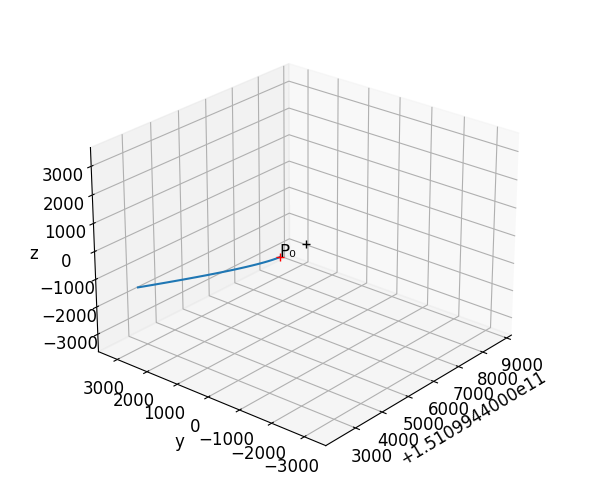
\includegraphics[scale=0.52]{figures/xyzplot1.png}
	\caption{Trajectory plot of an object near L2 fo the Sun-Earth system, x-coordinate is $(1.511\times10^{11} - 10^3)\si{\metre}$, all other conditions are 0.
		The red point, $P_0$, indicates the starting position of the object.
		The black point indicates the Lagrange point.
		Generated through the matplotlib and scipy Python libraries.
	}
	\label{fig:3dplot1}
\end{figure}
In order to create a trajectory that resembles an orbit, we need to apply velocity that is perpendicular to the acceleration to create circular motion.
Knowing that $v^2 = ar$, we can write the equation:
\begin{equation*}
	y_0' = k\sqrt{x''r}
\end{equation*}
where $y_0'$ is the initial velocity in the $y$ component and $k$ is the proportionality constant, assuming that the orbit being predicted is not actually circular.
After some trial and error, $k = 2.2$ makes for a good approximation.
\begin{figure}[H]
	\centering
	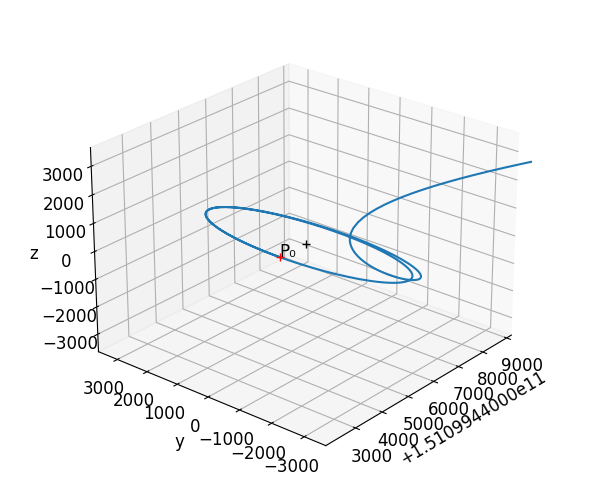
\includegraphics[scale=0.52]{figures/xyzplot2.png}
	\caption{Trajectory plot of an object $1000\si{\metre}$ in the proximity of L2 in the Sun-Earth system in a semi-stable halo orbit.}
	\label{fig:3dplot2}
\end{figure}
\end{samepage}
And would you look at that; in Figure \ref{fig:3dplot2}, it seems as if our satellite orbits nothing!
Of course, it is also seen that the satellite eventually falls out of its orbit, confirming the instability of collinear Lagrange points.

We can now use this model and compare it to the actual trajectory of objects orbiting Lagrange points.
Given that telemetry of the JWST is readily available through JPL Horizons System, we will use its orbit for comparison.
\begin{figure}[H]
	\centering
	\captionsetup[subfigure]{justification=centering}
	\begin{subfigure}[b]{0.4\textwidth}
		\centering
		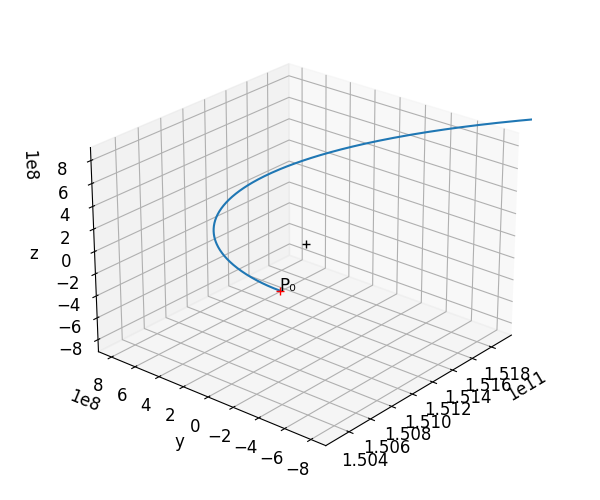
\includegraphics[scale=0.46]{figures/xyzplot3.png}
		\caption{Modelled trajectory plot of the JWST $2.5\times10^8\si{\metre}$ L2. Not modelled with station-keeping.}
		\label{fig:3dplot3}
	\end{subfigure}
	\qquad
	\begin{subfigure}[b]{0.4\textwidth}
		\centering
		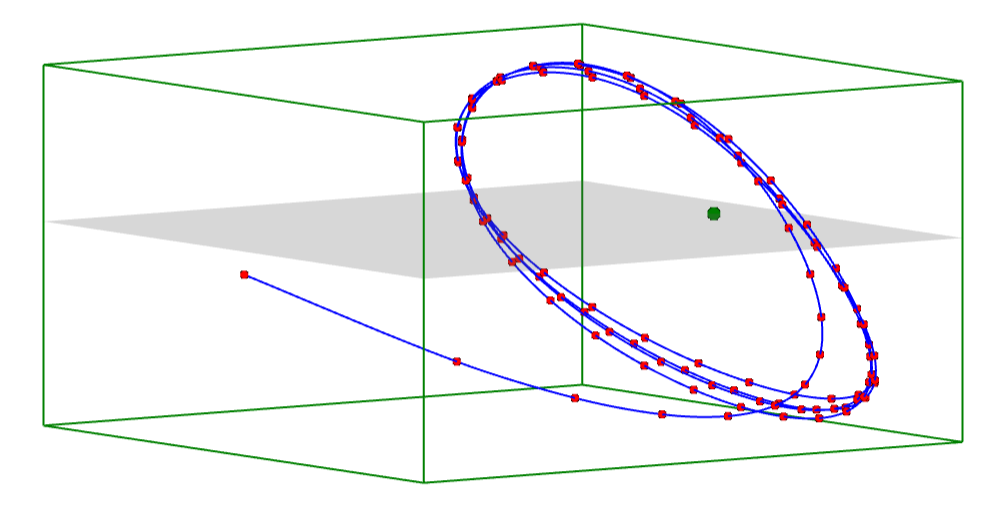
\includegraphics[scale=0.2]{figures/xyjwstplot.png}
		\vspace*{1em}
		\caption{Trajectory of the JWST according to the JPL Horizons database.}
		\label{fig:3dplot4}
		\vspace*{1em}
	\end{subfigure}
	\caption{Trajectories of the JWST. Figure (a) has $P_0$ positioned at $(L_2 - 2.5\times10^8, 0, - 1.2\times10^8)$. Figure (b) is generated through SageMath and produced by PM 2Ring on Stack Exchange.}
\end{figure}
Figure \ref{fig:3dplot3} is the trajectory of the JWST given the expected orbital characteristics prior to launch\autocite{JWSTHaloOrbit}.
Figure \ref{fig:3dplot4} is the trajectory of the JWST according to the JPL Horizons database from December 26th, 2021 to January 22, 2024\autocite{SEHaloOrbit}.
In Figure \ref{fig:3dplot3}, it is apparent that objects in large orbits around Lagrange points will ``fall off'' their orbits sooner than in a smaller orbit.
Therefore, it outlines the importance of station-keeping, where thrusters can be used to keep an object in its orbit, which is not considered in our model but is crucial for the JWST.
Still, the model seems to tend towards a similar elliptical, halo-like orbit that is shown in Figure \ref{fig:3dplot4}, indicating some accuracy.
The difference in trajectories in both figures can be attributed to the degree of sophistication between our model and the model used by JPL.
This can include consideration for an elliptical, eccentric orbit of the Earth, the effects of the Moon's gravity, and orbital eccentricity of the JWST during its transfer to L2.